\documentclass[journal]{IEEEtran}
\usepackage[a5paper, margin=10mm]{geometry}
%\usepackage{lmodern} % Ensure lmodern is loaded for pdflatex
\usepackage{tfrupee} % Include tfrupee package

\setlength{\headheight}{1cm}
\setlength{\headsep}{0mm}

\usepackage{gvv-book}
\usepackage{gvv}
\usetikzlibrary{patterns}
\lstset{aboveskip=12pt}
\usepackage[center]{caption}
\raggedbottom

\hypersetup{
    colorlinks=true,
    urlcolor=black
}
\usepackage{amsfonts}
\makeindex

\begin{document}
\bibliographystyle{IEEEtran}
\onecolumn

\title{
    \begin{center}
        Math for EE
        \\
        \rule{0.4\columnwidth}{0.4pt}
    \end{center}
}
\author{
    \vspace{11cm}
    \begin{center}
        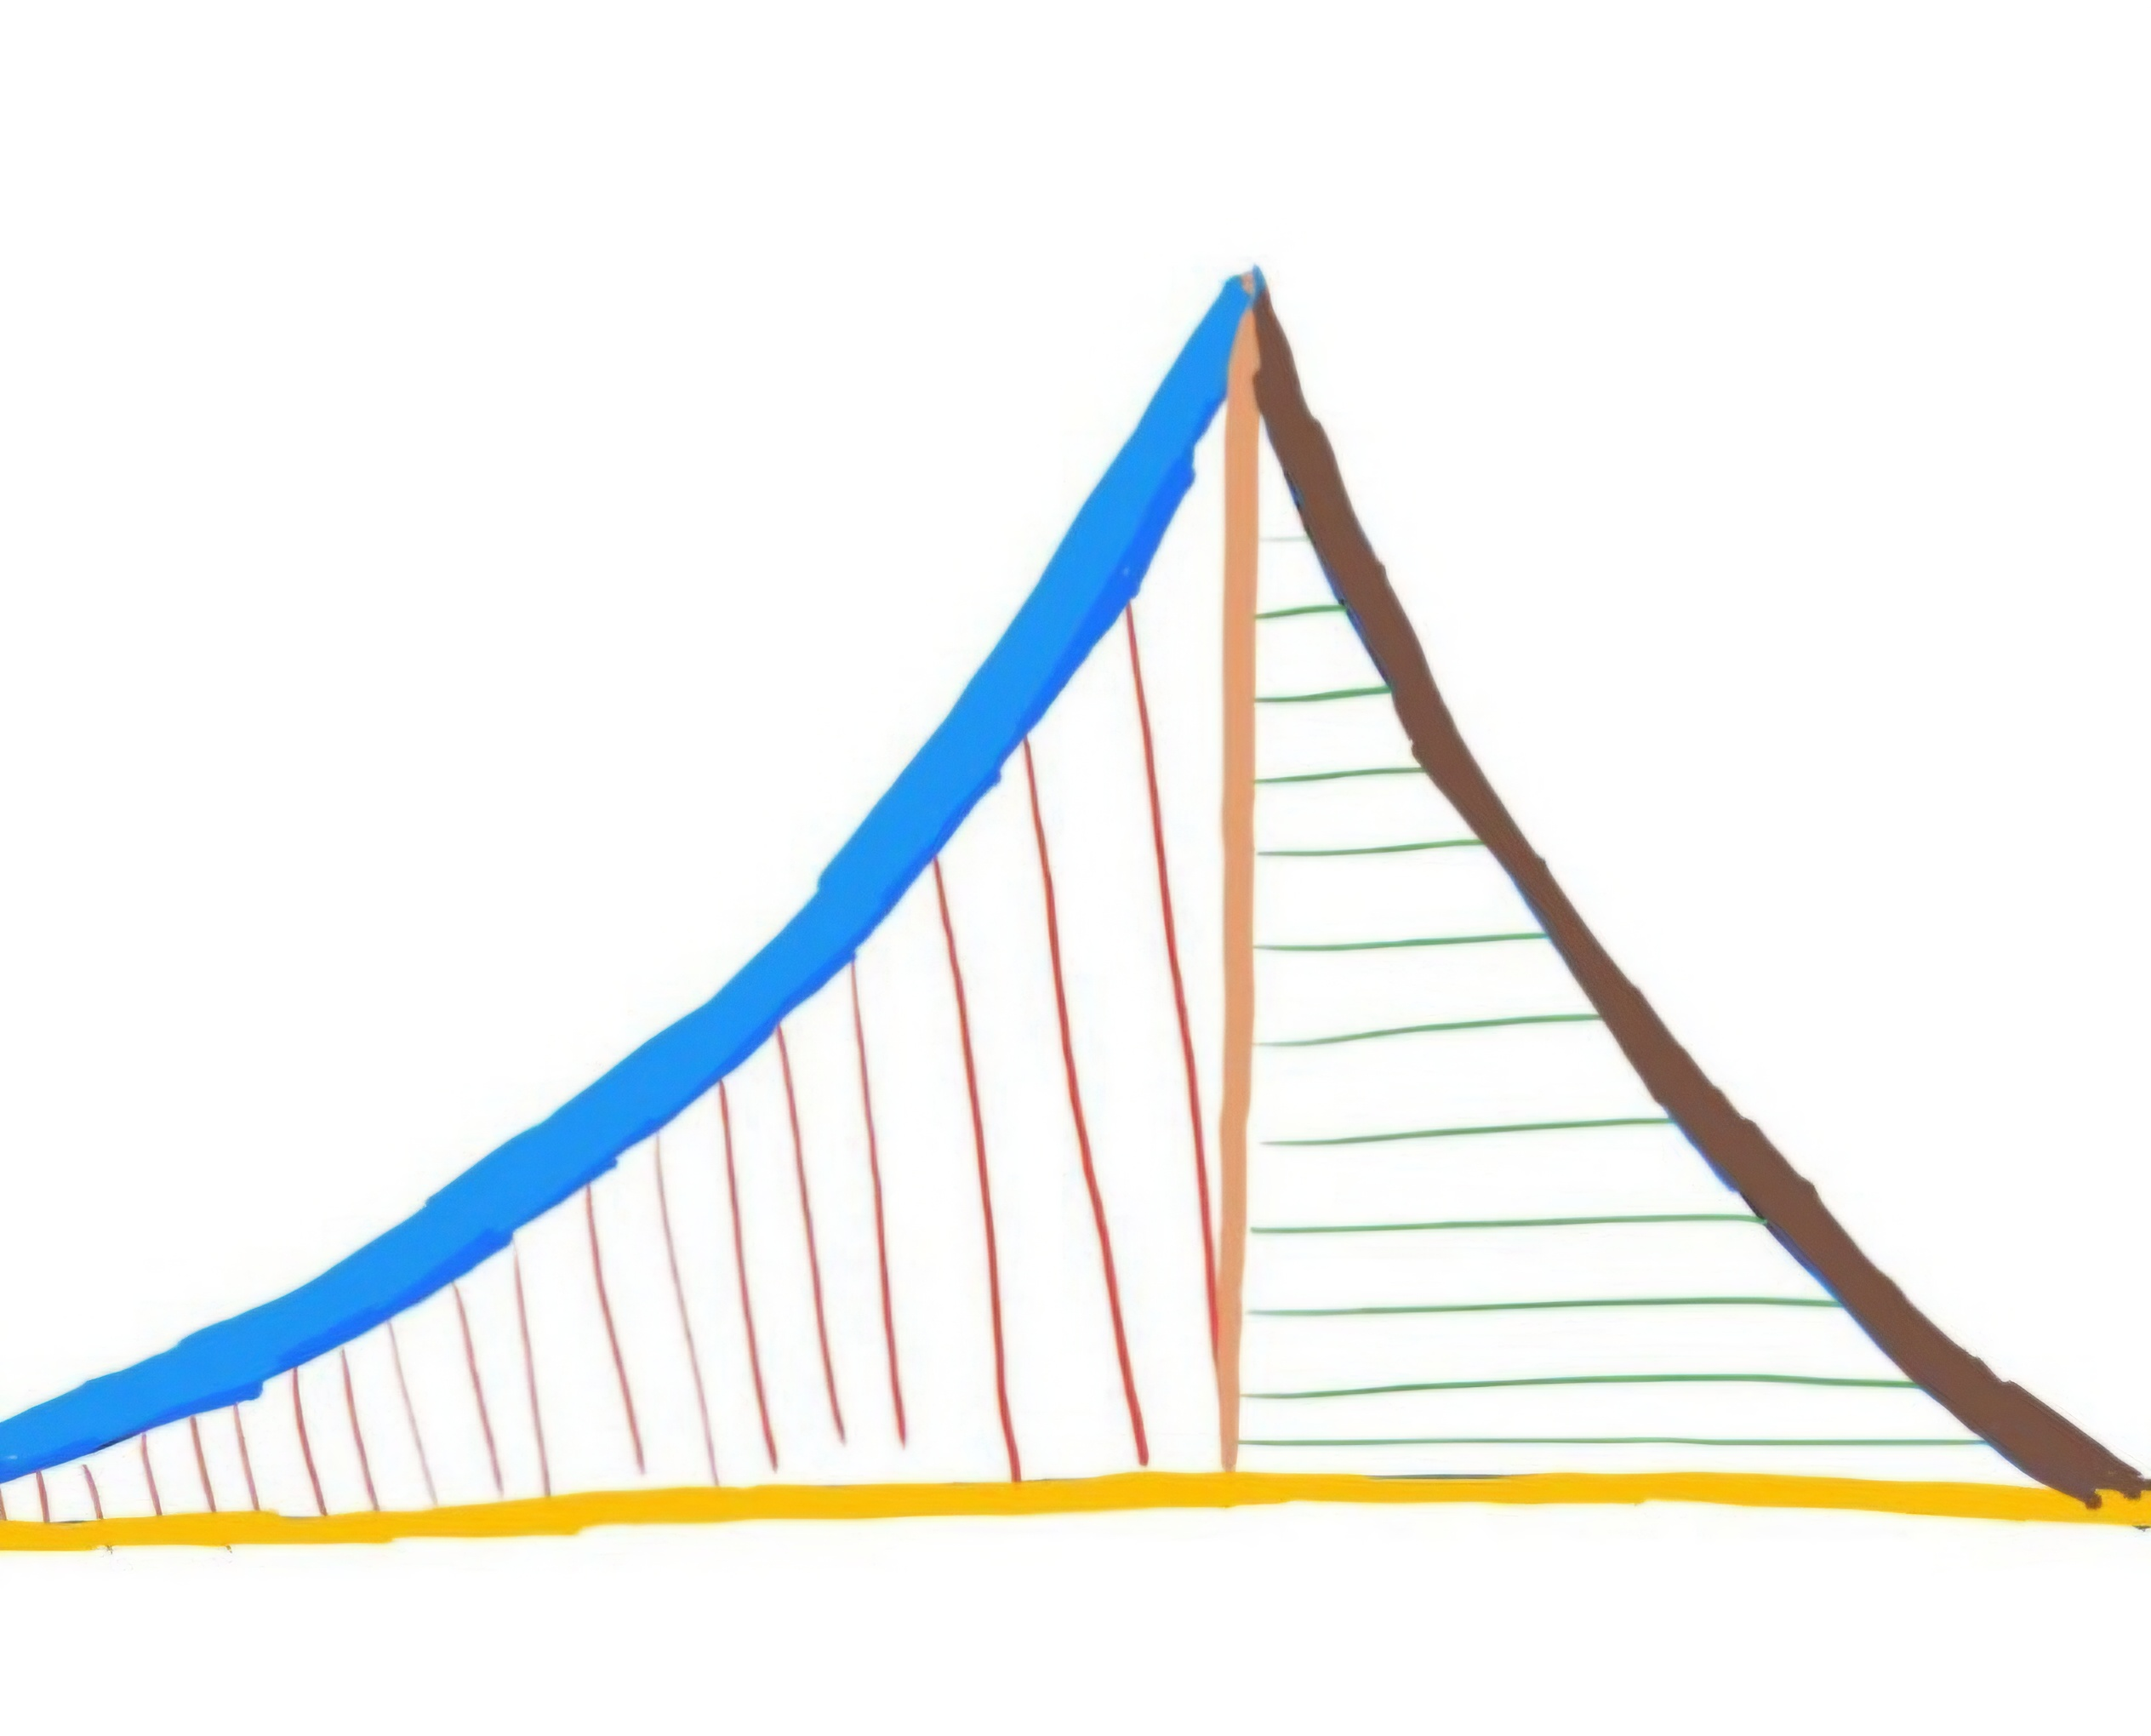
\includegraphics[width=0.2\columnwidth]{figs/logo.jpg}
        \\
        {\huge G. V. V. Sharma}
    \end{center}
}
\maketitle

\newpage
\section*{About this Book}

This book introduces matrices through high school coordinate geometry.
This approach makes it easier for beginners to learn Python for scientific
computing. All problems in the book are from NCERT mathematics textbooks
from Class 9--12. Exercises are from CBSE board exam papers.

The content is sufficient for industry jobs and covers nearly all matrix
prerequisites for machine learning. There is no copyright, so readers are
free to print and share.
License: https://creativecommons.org/licenses/by-sa/3.0/
\\
and
\\
https://www.gnu.org/licenses/fdl-1.3.en.html
\\
First manual appeared in January 2018
\\
First edition published on July 10, 2024
\\
In this edition, some incorrect solutions were removed. All figures
redrawn. More problems added.

\newpage
\onecolumn
\begin{center}
{\Large\bfseries CBSE 2026 12th class maths solutions (65-4-1)}
\end{center}
\vspace{0.4em}

\begin{list}{}{\setlength{\leftmargin}{1.15cm}\setlength{\labelwidth}{1.0cm}\setlength{\labelsep}{0.15cm}\setlength{\itemindent}{0pt}\setlength{\listparindent}{0pt}\setlength{\itemsep}{\baselineskip}\setlength{\parsep}{0pt}\setlength{\topsep}{0pt}}
\item[4.1.2] If $A=[a_{ij}]$ is a $2\times2$ matrix whose elements are given by $a_{ij}=\frac{|i-3j|}{2}$, then $A'$ is:

\noindent (A) $\begin{bmatrix}1&\frac{5}{2}\\[2pt]\frac{1}{2}&2\end{bmatrix}$ \hfill
(B) $\begin{bmatrix}1&\frac{1}{2}\\[2pt]\frac{5}{2}&2\end{bmatrix}$ \hfill
(C) $\begin{bmatrix}2&\frac{5}{2}\\[2pt]\frac{1}{2}&1\end{bmatrix}$ \hfill
(D) $\begin{bmatrix}2&\frac{1}{2}\\[2pt]\frac{5}{2}&1\end{bmatrix}$

\vspace{0.6em}\par\noindent\textbf{Solution:}

For $i,j\in\{1,2\}$, the entries are
\[
\begin{aligned}
a_{11}&=\frac{|1-3|}{2}=1, & a_{12}&=\frac{|1-6|}{2}=\frac52,\\
a_{21}&=\frac{|2-3|}{2}=\frac12, & a_{22}&=\frac{|2-6|}{2}=2.
\end{aligned}
\]
Thus $A=\begin{bmatrix}1&\frac52\\[2pt]\frac12&2\end{bmatrix}$, and its transpose is
\[
A'=\begin{bmatrix}1&\frac12\\[2pt]\frac52&2\end{bmatrix}.
\]
Therefore the correct answer is \textbf{(B)}.

\item[4.1.4] If the points $(2,3)$, $(0,4)$ and $(p,2)$ are collinear, find $p$.

\noindent (A) $\frac47$ \hfill (B) $-\frac37$ \hfill (C) $4$ \hfill (D) $-4$

\vspace{0.6em}\par\noindent\textbf{Solution:}

The slope through $(2,3)$ and $(0,4)$ is $-\frac12$. Collinearity requires $\frac{2-4}{p-0}=-\frac12$, giving $\boxed{p=4}$, option \textbf{(C)}. The Python program plots the three points and their common line.
\begin{lstlisting}[frame=single, basicstyle=\rmfamily, escapeinside={(*@}{@*)}]
(*@\makebox[\dimexpr\linewidth-2\fboxsep-2\fboxrule\relax][c]{codes/4.1.4.py}@*)
\end{lstlisting}
\begin{figure}[H]
\centering
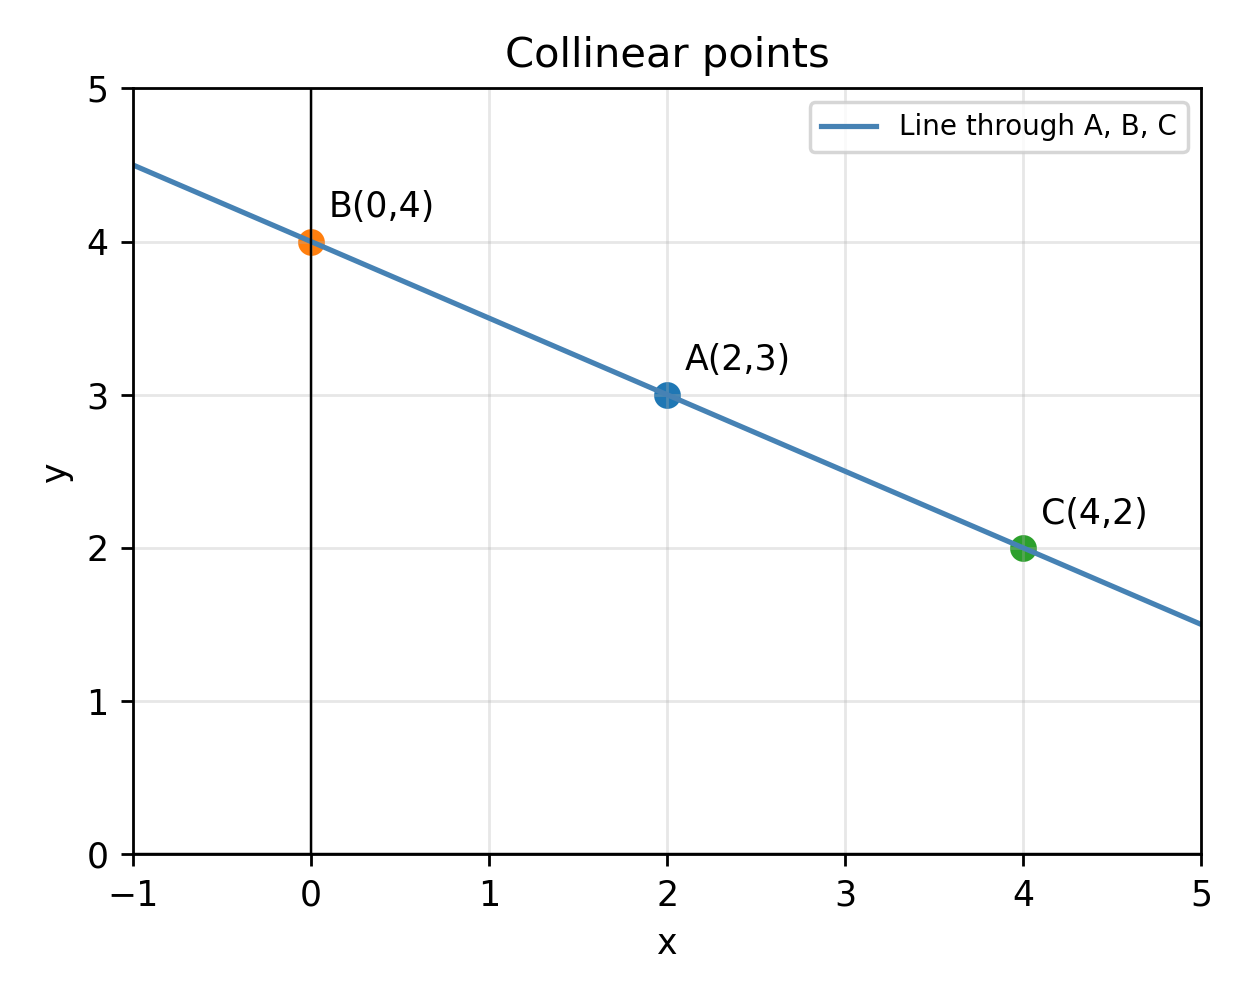
\includegraphics[width=0.65\linewidth]{figs/4.1.4.png}
\caption{The three collinear points for $p=4$.}
\end{figure}

\item[4.1.5] Find the differential of $e^{e^x}$ with respect to $x$.

\noindent (A) $\log x$ \hfill (B) $e^{e^x}$ \hfill (C) $e^xe^{e^x}$ \hfill (D) $(e^x)^2$

\vspace{0.6em}\par\noindent\textbf{Solution:}

By the chain rule, $\frac{d}{dx}e^{e^x}=e^{e^x}\cdot e^x$. Thus the answer is $\boxed{e^xe^{e^x}}$, option \textbf{(C)}. The Python code evaluates the derivative symbolically.
\begin{lstlisting}[frame=single, basicstyle=\rmfamily, escapeinside={(*@}{@*)}]
(*@\makebox[\dimexpr\linewidth-2\fboxsep-2\fboxrule\relax][c]{codes/4.1.5.py}@*)
\end{lstlisting}

\item[4.1.7] If $f(x)=\frac{\sin x}{x}+\cos x$ for $x\ne0$ and $f(0)=k$ is continuous at $x=0$, find $k$.

\noindent (A) $0$ \hfill (B) $-2$ \hfill (C) $-1$ \hfill (D) $2$

\vspace{0.6em}\par\noindent\textbf{Solution:}

$\lim_{x\to0}\left(\frac{\sin x}{x}+\cos x\right)=1+1=2$. Continuity requires $k$ to equal this limit, so $\boxed{k=2}$, option \textbf{(D)}. The plot shows the limiting value at the origin.
\begin{lstlisting}[frame=single, basicstyle=\rmfamily, escapeinside={(*@}{@*)}]
(*@\makebox[\dimexpr\linewidth-2\fboxsep-2\fboxrule\relax][c]{codes/4.1.7.py}@*)
\end{lstlisting}
\begin{figure}[H]
\centering
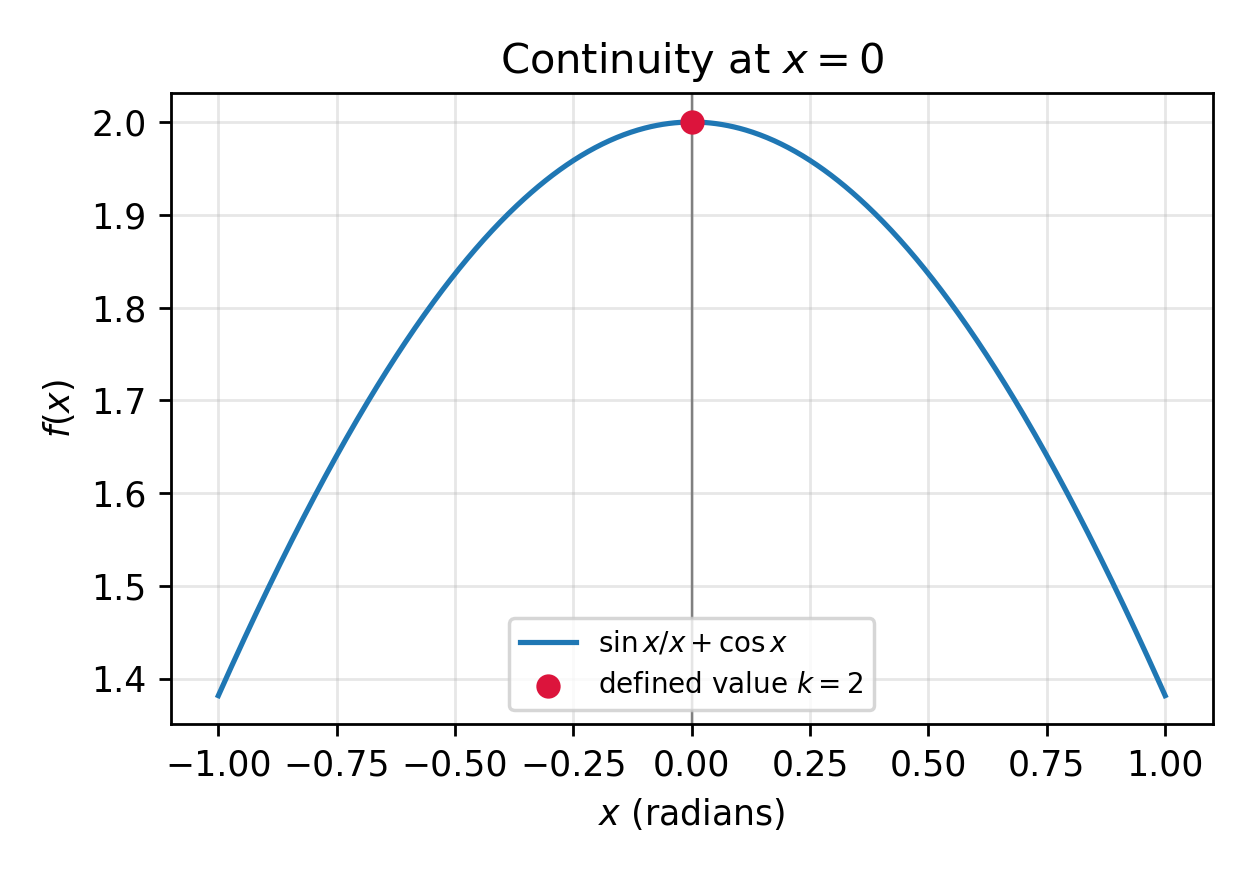
\includegraphics[width=0.65\linewidth]{figs/4.1.7.png}
\caption{The function approaches $2$ as $x$ approaches $0$.}
\end{figure}

\item[4.1.8] The greatest integer function $f(x)=[x]$, $0<x<3$, is not differentiable at how many points?

\noindent (A) Only one \hfill (B) Only two \hfill (C) None \hfill (D) Three

\vspace{0.6em}\par\noindent\textbf{Solution:}

The function has jump discontinuities at the integers $x=1$ and $x=2$ in this open interval. A discontinuous function cannot be differentiable there. Hence it is not differentiable at $\boxed{2}$ points, option \textbf{(B)}.

\item[4.1.9] Evaluate $\displaystyle\int\frac{dx}{\sqrt{25-16x^2}}$.

\noindent (A) $\frac15\sin^{-1}(4x)+C$ \hfill (B) $\frac1{25}\sin^{-1}(16x)+C$ \\
(C) $\frac14\sin^{-1}\left(\frac{4x}{5}\right)+C$ \hfill (D) $\frac1{16}\sin^{-1}\left(\frac{4x}{5}\right)+C$

\vspace{0.6em}\par\noindent\textbf{Solution:}

Factor the radicand as $25\left(1-(4x/5)^2\right)$. With $u=4x/5$, the integral becomes $\frac14\int\frac{du}{\sqrt{1-u^2}}$, so the result is $\boxed{\frac14\sin^{-1}(4x/5)+C}$, option \textbf{(C)}.

\item[4.1.11] Find the area bounded by $y=x$, the $x$-axis, and $x=0$ to $x=2$.

\vspace{0.6em}\par\noindent\textbf{Solution:}

The required area is $\int_0^2x\,dx=\left[x^2/2\right]_0^2=\boxed{2}$ square units. The code plots the lines and shades the bounded region.
\begin{lstlisting}[frame=single, basicstyle=\rmfamily, escapeinside={(*@}{@*)}]
(*@\makebox[\dimexpr\linewidth-2\fboxsep-2\fboxrule\relax][c]{codes/4.1.11.py}@*)
\end{lstlisting}
\begin{figure}[H]
\centering
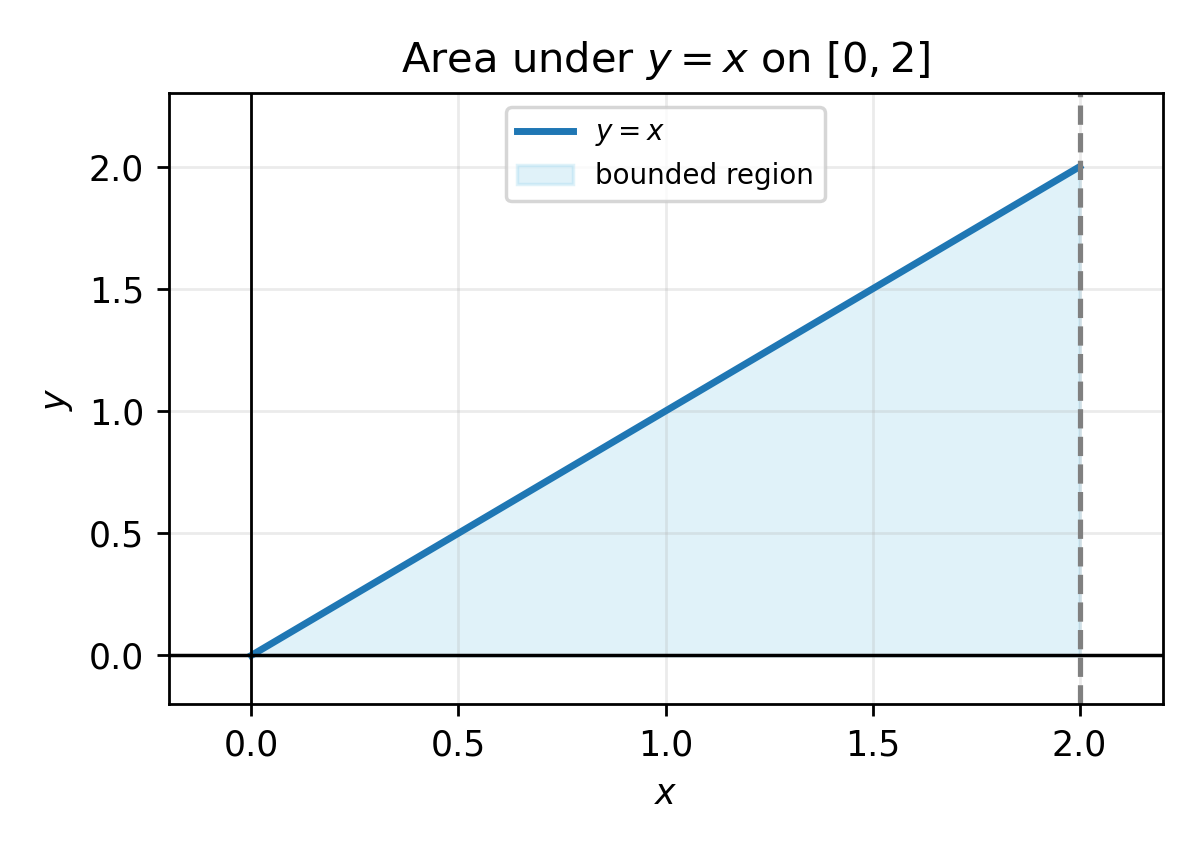
\includegraphics[width=0.65\linewidth]{figs/4.1.11.png}
\caption{Area under $y=x$ on $0\le x\le2$.}
\end{figure}

\item[4.1.14] Identify the region represented by $3x+y\ge3$, $2x-y\ge-5$, $x,y\ge0$.

\noindent (A) Unbounded in the first quadrant \hfill (B) Bounded in the first quadrant \\
(C) Unbounded in the second quadrant \hfill (D) Bounded in the second quadrant

\vspace{0.6em}\par\noindent\textbf{Solution:}

The conditions $x,y\ge0$ place the region in the first quadrant. The boundary lines are $y=3-3x$ and $y=2x+5$; the feasible region extends indefinitely as $x$ increases. It is therefore \textbf{unbounded in the first quadrant}, option \textbf{(A)}. The code plots the boundaries and shades the feasible region.
\begin{lstlisting}[frame=single, basicstyle=\rmfamily, escapeinside={(*@}{@*)}]
(*@\makebox[\dimexpr\linewidth-2\fboxsep-2\fboxrule\relax][c]{codes/4.1.14.py}@*)
\end{lstlisting}
\begin{figure}[H]
\centering
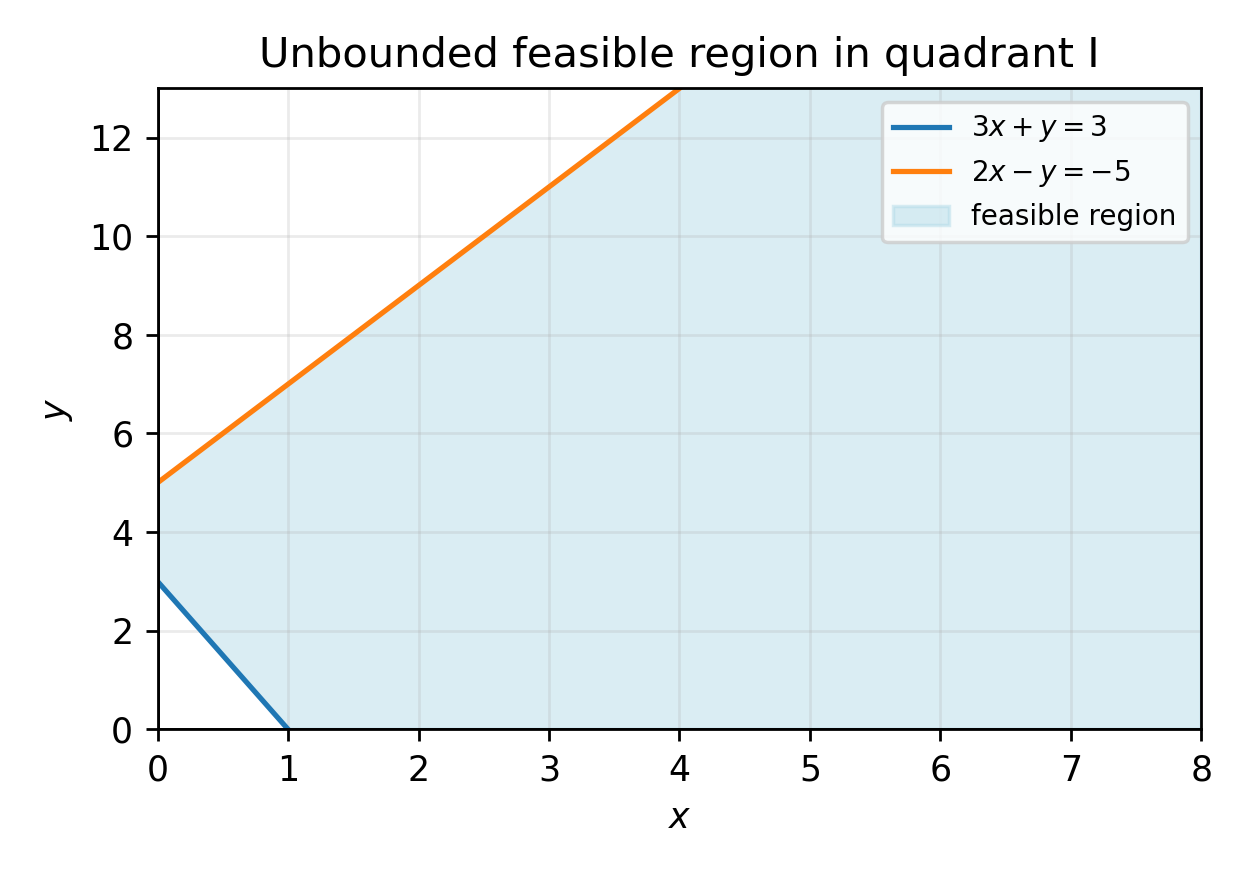
\includegraphics[width=0.65\linewidth]{figs/4.1.14.png}
\caption{Unbounded feasible region for Question 14.}
\end{figure}

\item[4.1.15] In the given graph, every point on segment $AB$ maximizes $Z=px+qy$, $p,q>0$. Determine the relation between $p$ and $q$.

\noindent (A) $p=2q$ \hfill (B) $p=3q$ \hfill (C) $q=3p$ \hfill (D) $q=2p$

\vspace{0.6em}\par\noindent\textbf{Solution:}

From the graph, $A=(0,5)$ and $B=(3,4)$, so the slope of $AB$ is $-1/3$. The objective lines have slope $-p/q$. For all points on $AB$ to be optimal, these slopes must match: $-p/q=-1/3$, hence $\boxed{q=3p}$, option \textbf{(C)}. The code plots $AB$ and a parallel objective line.
\begin{lstlisting}[frame=single, basicstyle=\rmfamily, escapeinside={(*@}{@*)}]
(*@\makebox[\dimexpr\linewidth-2\fboxsep-2\fboxrule\relax][c]{codes/4.1.15.py}@*)
\end{lstlisting}
\begin{figure}[H]
\centering
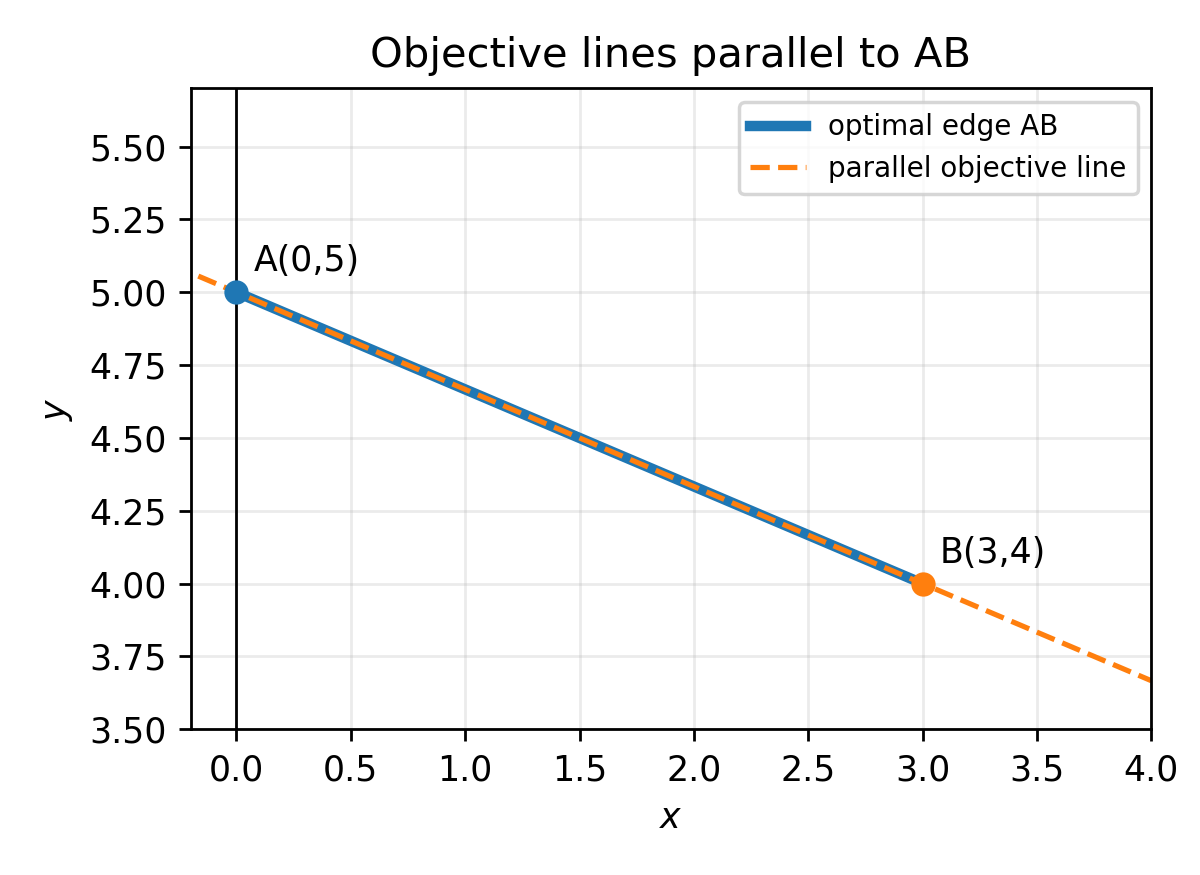
\includegraphics[width=0.65\linewidth]{figs/4.1.15.png}
\caption{The objective line is parallel to the optimal edge $AB$.}
\end{figure}

\item[4.1.17] Find the area of the triangle with vertices $A(0,1,1)$, $B(2,0,-1)$ and $C(1,0,3)$.

\noindent (A) $\frac{\sqrt{53}}2$ \hfill (B) $\sqrt{53}$ \hfill (C) $\frac{\sqrt{11}}2$ \hfill (D) $\sqrt{11}$

\vspace{0.6em}\par\noindent\textbf{Solution:}

$\overrightarrow{AB}=(2,-1,-2)$ and $\overrightarrow{AC}=(1,-1,2)$. Their cross product has magnitude $\sqrt{53}$, so $\operatorname{ar}(\triangle ABC)=\frac12|\overrightarrow{AB}\times\overrightarrow{AC}|=\boxed{\frac{\sqrt{53}}2}$ square units, option \textbf{(A)}. The code plots the triangle and computes its area.
\begin{lstlisting}[frame=single, basicstyle=\rmfamily, escapeinside={(*@}{@*)}]
(*@\makebox[\dimexpr\linewidth-2\fboxsep-2\fboxrule\relax][c]{codes/4.1.17.py}@*)
\end{lstlisting}
\begin{figure}[H]
\centering
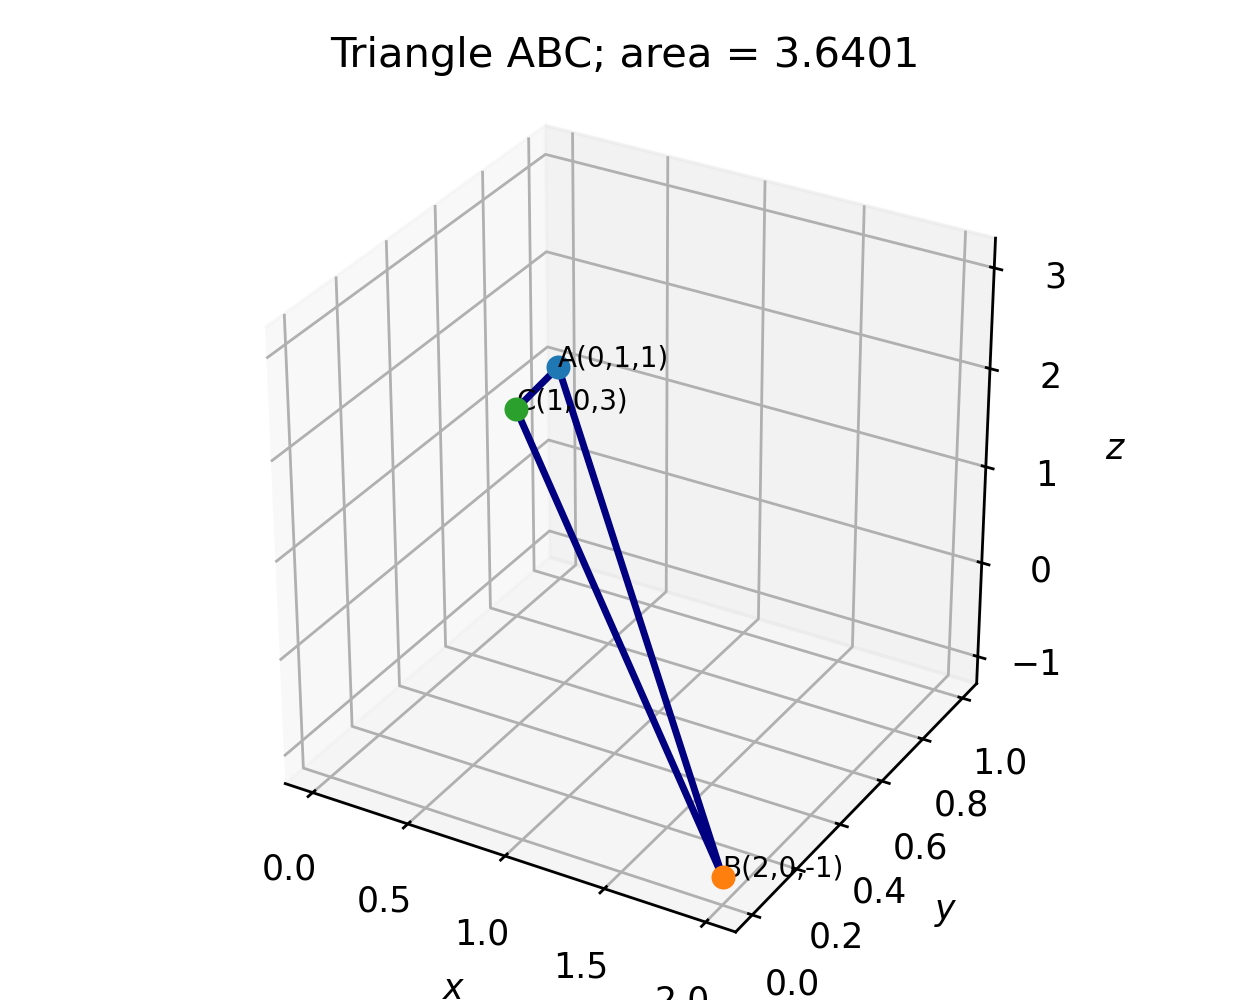
\includegraphics[width=0.65\linewidth]{figs/4.1.17.png}
\caption{Triangle $ABC$ in three-dimensional space.}
\end{figure}

\item[4.1.18] A box contains 4 red, 5 blue and 1 green marble. A marble is drawn and replaced, and this is repeated three times. Find the probability of at least one red marble.

\noindent (A) $\frac{27}{125}$ \hfill (B) $\frac{8}{125}$ \hfill (C) $\frac{2}{125}$ \hfill (D) $\frac{98}{125}$

\vspace{0.6em}\par\noindent\textbf{Solution:}

Use the complement: the probability of no red marble in one draw is $6/10=3/5$. Thus $P(\text{at least one red})=1-(3/5)^3=\boxed{98/125}$, option \textbf{(D)}.

\item[4.1.20] Assertion (A): $f:\mathbb{N}\to\mathbb{N}$, $f(x)=x^3+2$, is one-one but not onto. Reason (R): For every $y\in\mathbb{N}$ there is no $x\in\mathbb{N}$ with $x^3+2=y$.

\vspace{0.6em}\par\noindent\textbf{Solution:}

The graph on the natural-number domain is strictly increasing, so $f$ is one-one; it is not onto because its values start at $3$ and omit natural numbers such as $1$. The reason is false as stated: for example, $y=3$ has preimage $x=1$. Therefore Assertion is true and Reason is false, option \textbf{(C)}. The plotted values illustrate the image of $f$.
\begin{lstlisting}[frame=single, basicstyle=\rmfamily, escapeinside={(*@}{@*)}]
(*@\makebox[\dimexpr\linewidth-2\fboxsep-2\fboxrule\relax][c]{codes/4.1.20.py}@*)
\end{lstlisting}
\begin{figure}[H]
\centering
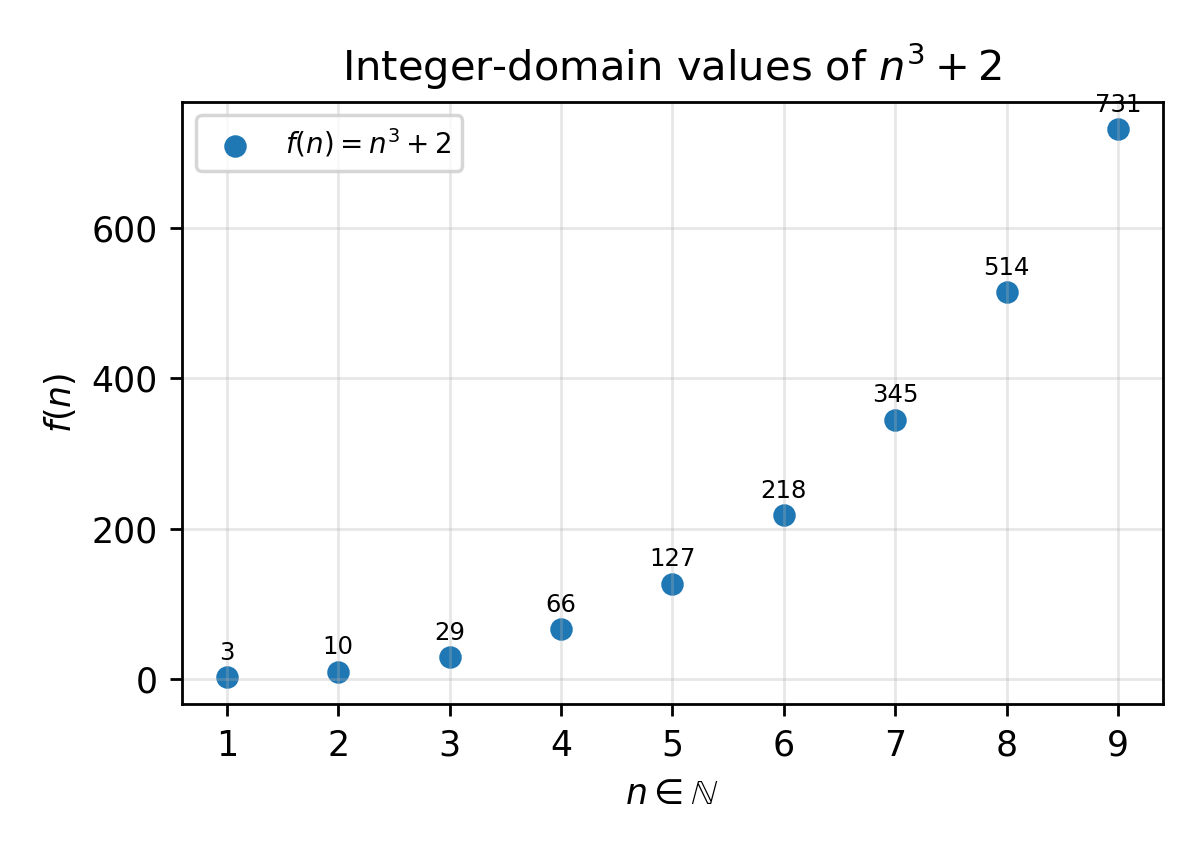
\includegraphics[width=0.65\linewidth]{figs/4.1.20.png}
\caption{Values of $n^3+2$ for natural-number inputs.}
\end{figure}

\item[4.1.22(a)] Show that $f(x)=\frac{\cos x}{\frac\pi2-x}$ for $x\ne\frac\pi2$, and $f(\frac\pi2)=1$, is continuous at $x=\frac\pi2$.

\vspace{0.6em}\par\noindent\textbf{Solution:}

Put $h=\frac\pi2-x$. Then $\cos x=\sin h$, so $\lim_{x\to\pi/2}f(x)=\lim_{h\to0}\frac{\sin h}{h}=1=f(\frac\pi2)$. Hence $f$ is continuous there. The code plots the function and its defined value.
\begin{lstlisting}[frame=single, basicstyle=\rmfamily, escapeinside={(*@}{@*)}]
(*@\makebox[\dimexpr\linewidth-2\fboxsep-2\fboxrule\relax][c]{codes/4.1.22a.py}@*)
\end{lstlisting}
\begin{figure}[H]
\centering
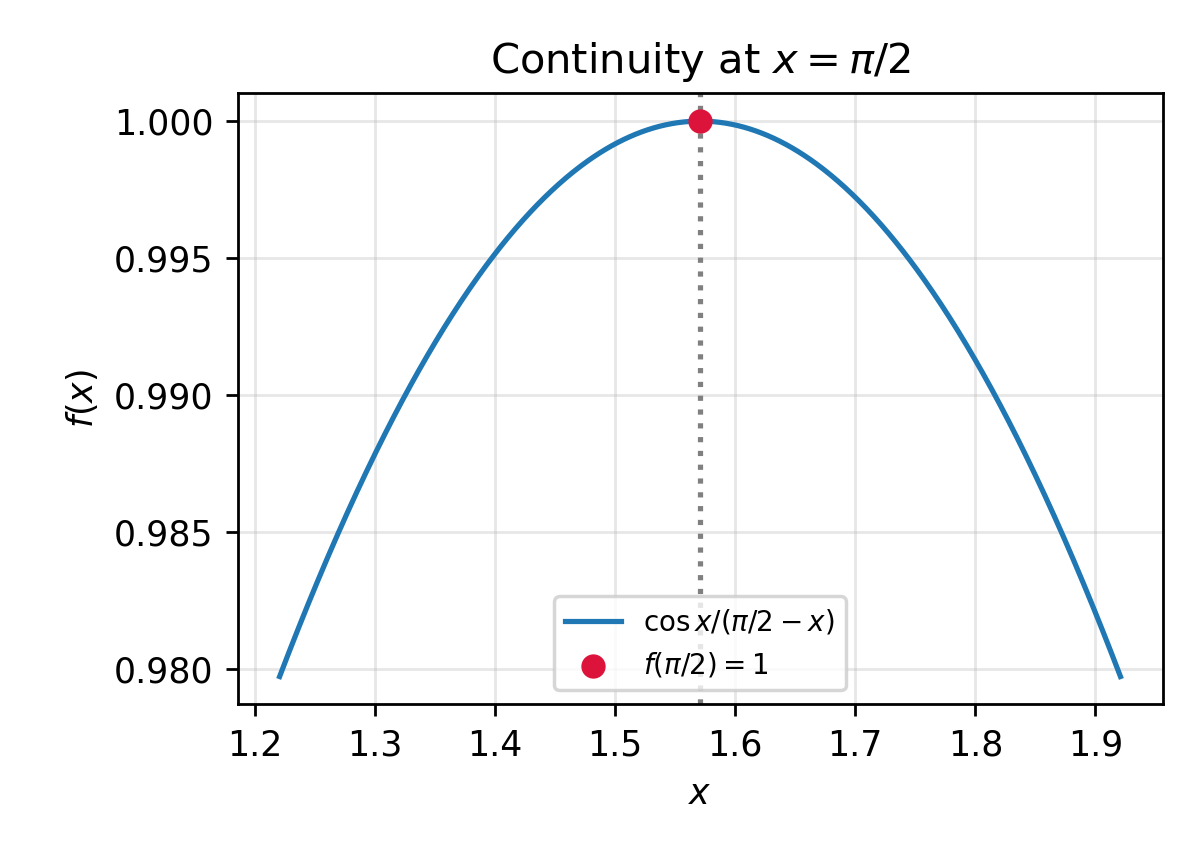
\includegraphics[width=0.65\linewidth]{figs/4.1.22a.png}
\caption{The limit and defined value meet at $x=\pi/2$.}
\end{figure}

\item[4.1.22(b)] Determine whether $f(x)=x-1$ for $x<2$ and $f(x)=2x-3$ for $x\ge2$ is differentiable at $x=2$.

\vspace{0.6em}\par\noindent\textbf{Solution:}

Both one-sided limits and $f(2)$ equal $1$, so the function is continuous at $2$. The left and right derivatives are respectively $1$ and $2$, which are unequal. Thus $f$ is \textbf{not differentiable} at $x=2$. The code plots the two branches.
\begin{lstlisting}[frame=single, basicstyle=\rmfamily, escapeinside={(*@}{@*)}]
(*@\makebox[\dimexpr\linewidth-2\fboxsep-2\fboxrule\relax][c]{codes/4.1.22b.py}@*)
\end{lstlisting}
\begin{figure}[H]
\centering
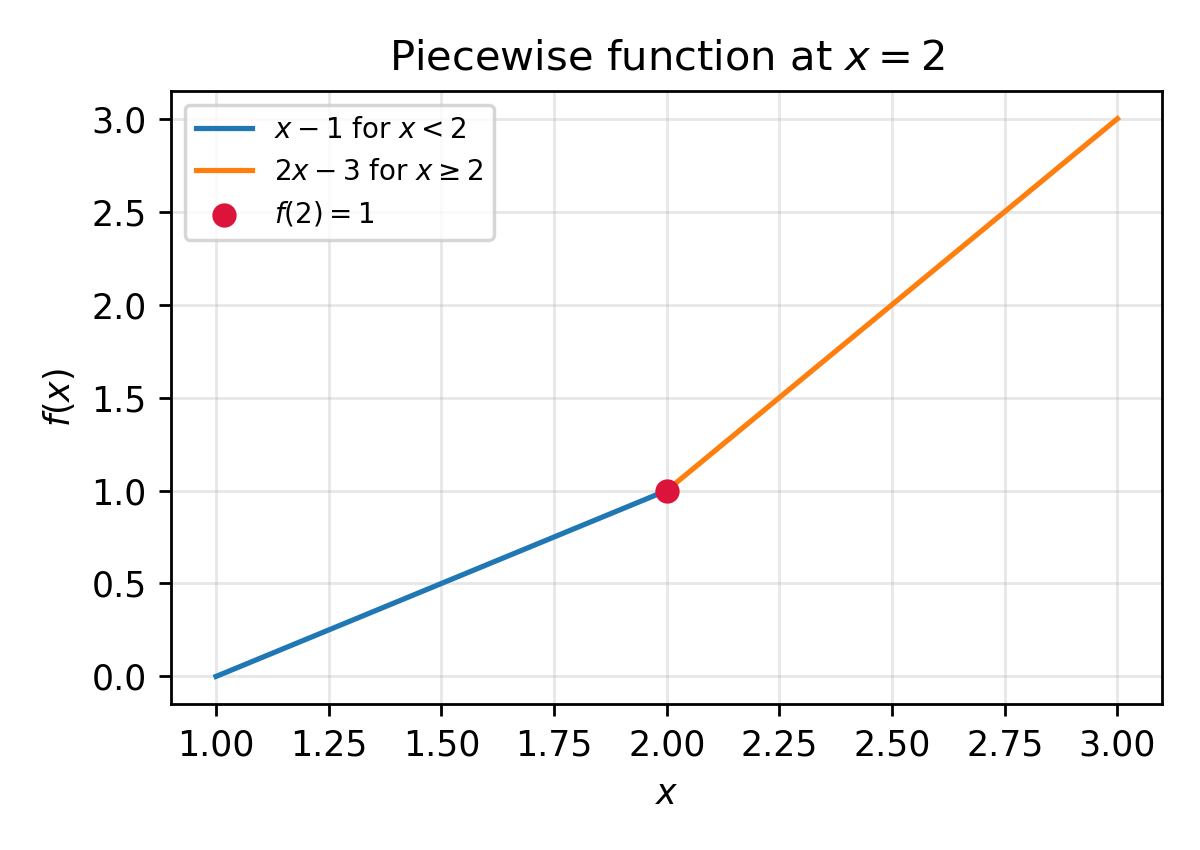
\includegraphics[width=0.65\linewidth]{figs/4.1.22b.png}
\caption{The two linear branches meet with different slopes at $x=2$.}
\end{figure}

\item[4.1.23] Find the values of $x$ for which $f(x)=x^x$, $x>0$, is increasing.

\vspace{0.6em}\par\noindent\textbf{Solution:}

Logarithmic differentiation gives $f'(x)=x^x(1+\ln x)$. Since $x^x>0$, the derivative is positive exactly when $1+\ln x>0$, or $\boxed{x>1/e}$. The graph and the code's derivative analysis show the change from decreasing to increasing at $x=1/e$.
\begin{lstlisting}[frame=single, basicstyle=\rmfamily, escapeinside={(*@}{@*)}]
(*@\makebox[\dimexpr\linewidth-2\fboxsep-2\fboxrule\relax][c]{codes/4.1.23.py}@*)
\end{lstlisting}
\begin{figure}[H]
\centering
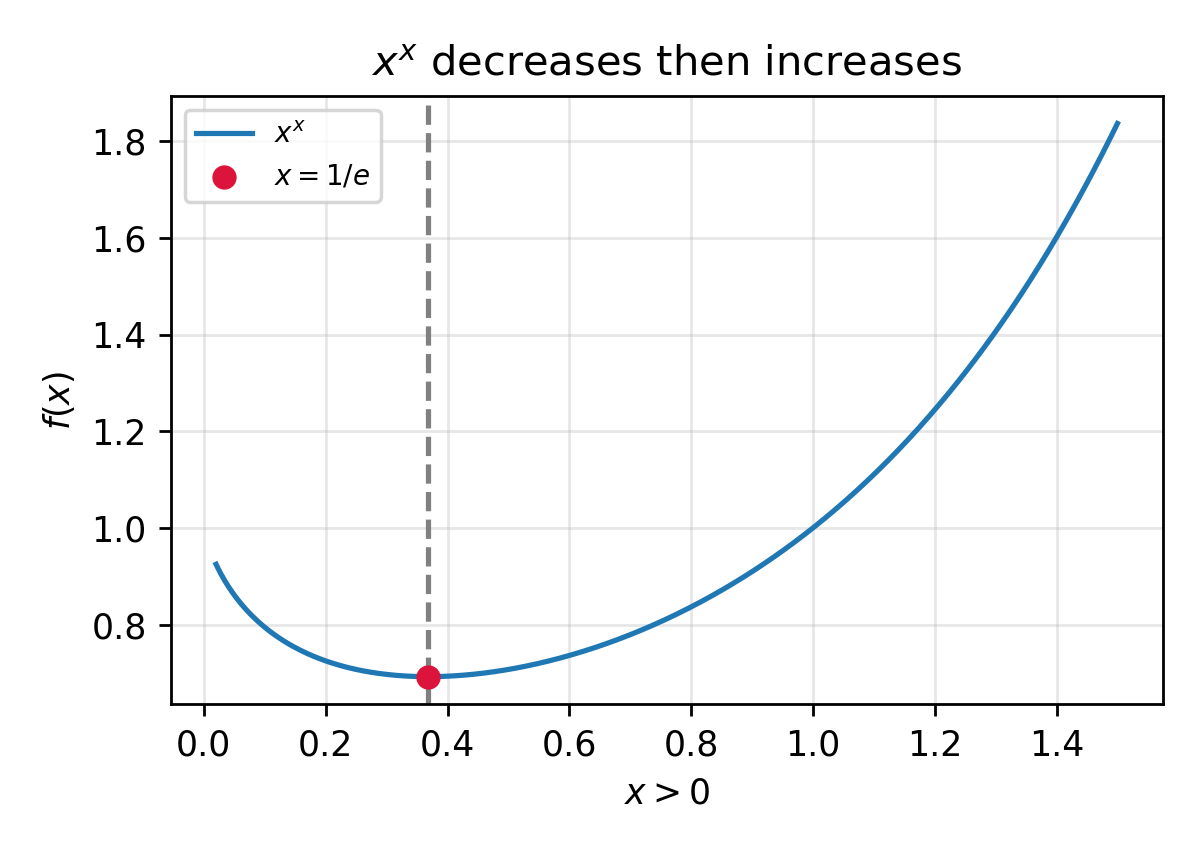
\includegraphics[width=0.65\linewidth]{figs/4.1.23.png}
\caption{The minimum of $x^x$ occurs at $x=1/e$.}
\end{figure}

\item[4.1.24] The position vectors of $A,B,C$ are $3\hat i+\hat j$, $5\hat i+6\hat j-3\hat k$, and $4\hat j$. Show that $ABC$ is isosceles.

\vspace{0.6em}\par\noindent\textbf{Solution:}

The corresponding points are $A(3,1,0)$, $B(5,6,-3)$ and $C(0,4,0)$. Their side lengths are $AB=\sqrt{38}$, $BC=\sqrt{38}$ and $AC=\sqrt{18}$. Therefore $AB=BC$, so $ABC$ is isosceles. The code uses the CoordGeo triangle side-length function and plots the triangle.
\begin{lstlisting}[frame=single, basicstyle=\rmfamily, escapeinside={(*@}{@*)}]
(*@\makebox[\dimexpr\linewidth-2\fboxsep-2\fboxrule\relax][c]{codes/4.1.24.py}@*)
\end{lstlisting}
\begin{figure}[H]
\centering
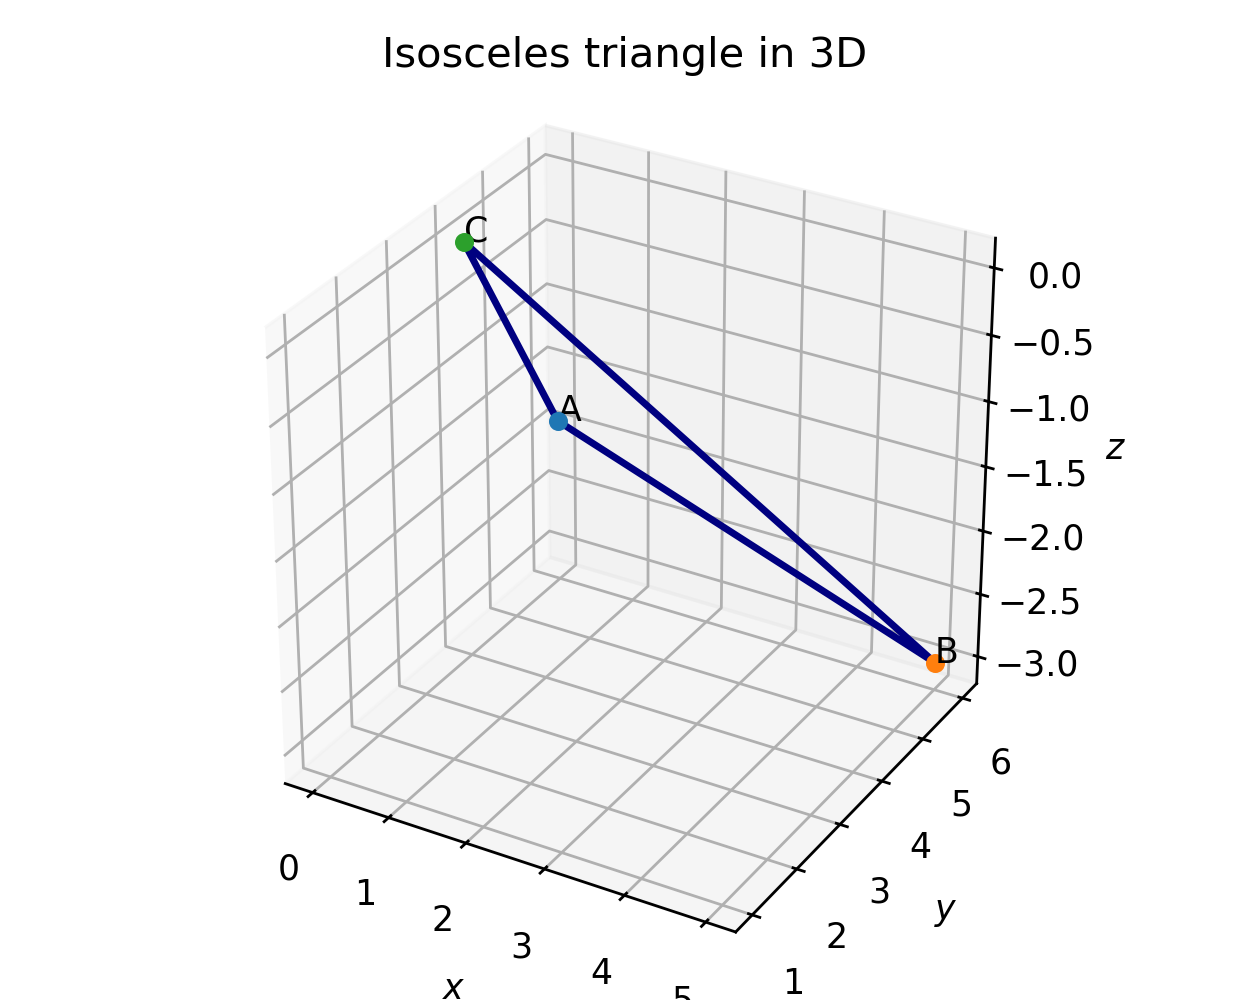
\includegraphics[width=0.65\linewidth]{figs/4.1.24.png}
\caption{The three vertices and equal sides of $\triangle ABC$.}
\end{figure}

\item[4.1.25(a)] Two rods are represented by $4\hat i-\hat j+3\hat k$ and $-2\hat i+\hat j-2\hat k$. Find a vector for a 5 m flag-post perpendicular to both.

\vspace{0.6em}\par\noindent\textbf{Solution:}

The cross product of the rod vectors is $(-1,2,2)$, of magnitude $3$. A perpendicular vector of magnitude $5$ is therefore $\boxed{\pm\frac53(-\hat i+2\hat j+2\hat k)\text{ m}}$. The code computes this vector and plots both rods and the flag-post.
\begin{lstlisting}[frame=single, basicstyle=\rmfamily, escapeinside={(*@}{@*)}]
(*@\makebox[\dimexpr\linewidth-2\fboxsep-2\fboxrule\relax][c]{codes/4.1.25a.py}@*)
\end{lstlisting}
\begin{figure}[H]
\centering
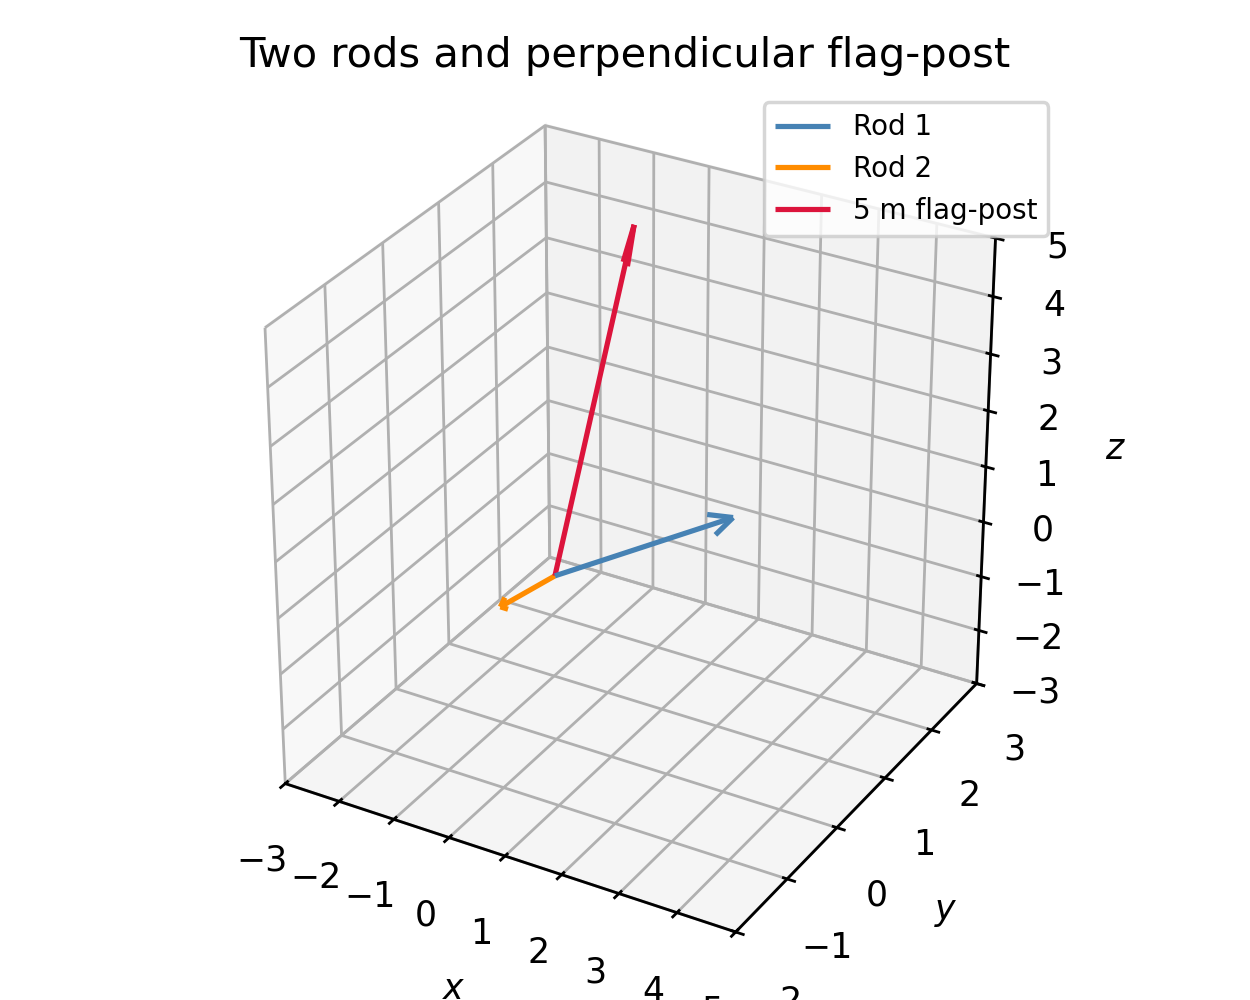
\includegraphics[width=0.65\linewidth]{figs/4.1.25a.png}
\caption{A 5 m vector perpendicular to both rod vectors.}
\end{figure}

\item[4.1.26] Let $A=\mathbb R\setminus\{3\}$, $B=\mathbb R\setminus\{1\}$ and $f:A\to B$ be $f(x)=\frac{x-2}{x-3}$. Determine whether $f$ is one-one and onto.

\vspace{0.6em}\par\noindent\textbf{Solution:}

If $y=\frac{x-2}{x-3}$, then $x=\frac{3y-2}{y-1}$. This inverse is defined for every $y\ne1$ and never equals $3$. Thus every element of $B$ has exactly one preimage in $A$: $f$ is both one-one and onto. The code plots the function and its excluded asymptotes.
\begin{lstlisting}[frame=single, basicstyle=\rmfamily, escapeinside={(*@}{@*)}]
(*@\makebox[\dimexpr\linewidth-2\fboxsep-2\fboxrule\relax][c]{codes/4.1.26.py}@*)
\end{lstlisting}
\begin{figure}[H]
\centering
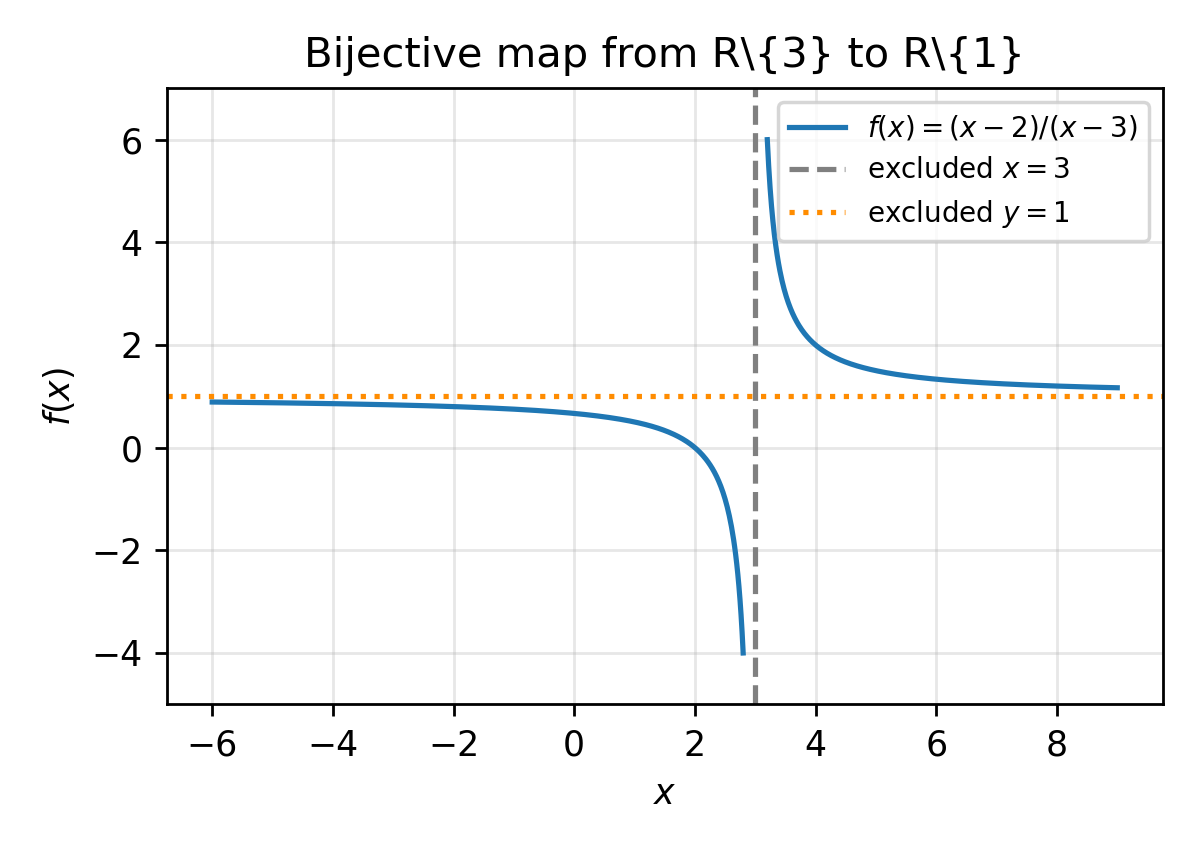
\includegraphics[width=0.65\linewidth]{figs/4.1.26.png}
\caption{The graph has excluded input $x=3$ and excluded output $y=1$.}
\end{figure}

\item[4.1.27] If $A=\begin{bmatrix}3&2&0\\1&4&0\\0&0&5\end{bmatrix}$, compute $A^2-7A+10I$.

\vspace{0.6em}\par\noindent\textbf{Solution:}

Direct matrix multiplication gives $A^2=\begin{bmatrix}11&14&0\\7&18&0\\0&0&25\end{bmatrix}$. Hence
\[
A^2-7A+10I=\boxed{\begin{bmatrix}0&0&0\\0&0&0\\0&0&0\end{bmatrix}}.
\]
The Python code carries out the matrix operation.
\begin{lstlisting}[frame=single, basicstyle=\rmfamily, escapeinside={(*@}{@*)}]
(*@\makebox[\dimexpr\linewidth-2\fboxsep-2\fboxrule\relax][c]{codes/4.1.27.py}@*)
\end{lstlisting}

\item[4.1.28(a)] If $xy=e^{x-y}$, find $\frac{dy}{dx}$.

\vspace{0.6em}\par\noindent\textbf{Solution:}

Taking logarithms gives $\ln x+\ln y=x-y$. Differentiating and collecting the $y'$ terms yields $\boxed{\frac{dy}{dx}=\frac{y(x-1)}{x(y+1)}}$. The Python code solves the differentiated equation.
\begin{lstlisting}[frame=single, basicstyle=\rmfamily, escapeinside={(*@}{@*)}]
(*@\makebox[\dimexpr\linewidth-2\fboxsep-2\fboxrule\relax][c]{codes/4.1.28a.py}@*)
\end{lstlisting}

\item[4.1.28(b)] Differentiate $\tan^{-1}\!\left(\frac{\sqrt{1+x^2}-\sqrt{1-x^2}}{\sqrt{1+x^2}+\sqrt{1-x^2}}\right)$ with respect to $\cos^{-1}(x^2)$.

\vspace{0.6em}\par\noindent\textbf{Solution:}

Using the chain rule for the ratio of derivatives with respect to $x$ gives $\boxed{-\frac12}$ (for interior values where the derivatives are defined). The Python code differentiates and simplifies the expression symbolically.
\begin{lstlisting}[frame=single, basicstyle=\rmfamily, escapeinside={(*@}{@*)}]
(*@\makebox[\dimexpr\linewidth-2\fboxsep-2\fboxrule\relax][c]{codes/4.1.28b.py}@*)
\end{lstlisting}

\item[4.1.29] Maximize $Z=200x+120y$ subject to $x+y\le300$, $3x+y\le600$, $x-y\ge-100$, $x,y\ge0$.

\vspace{0.6em}\par\noindent\textbf{Solution:}

The feasible vertices are $(0,0)$, $(0,100)$, $(100,200)$, $(150,150)$ and $(200,0)$. The objective values there are $0$, $12000$, $44000$, $48000$ and $40000$. Therefore the maximum is $\boxed{Z=48000}$ at $(x,y)=\boxed{(150,150)}$. The code plots the constraints and computes the vertex values.
\begin{lstlisting}[frame=single, basicstyle=\rmfamily, escapeinside={(*@}{@*)}]
(*@\makebox[\dimexpr\linewidth-2\fboxsep-2\fboxrule\relax][c]{codes/4.1.29.py}@*)
\end{lstlisting}
\begin{figure}[H]
\centering
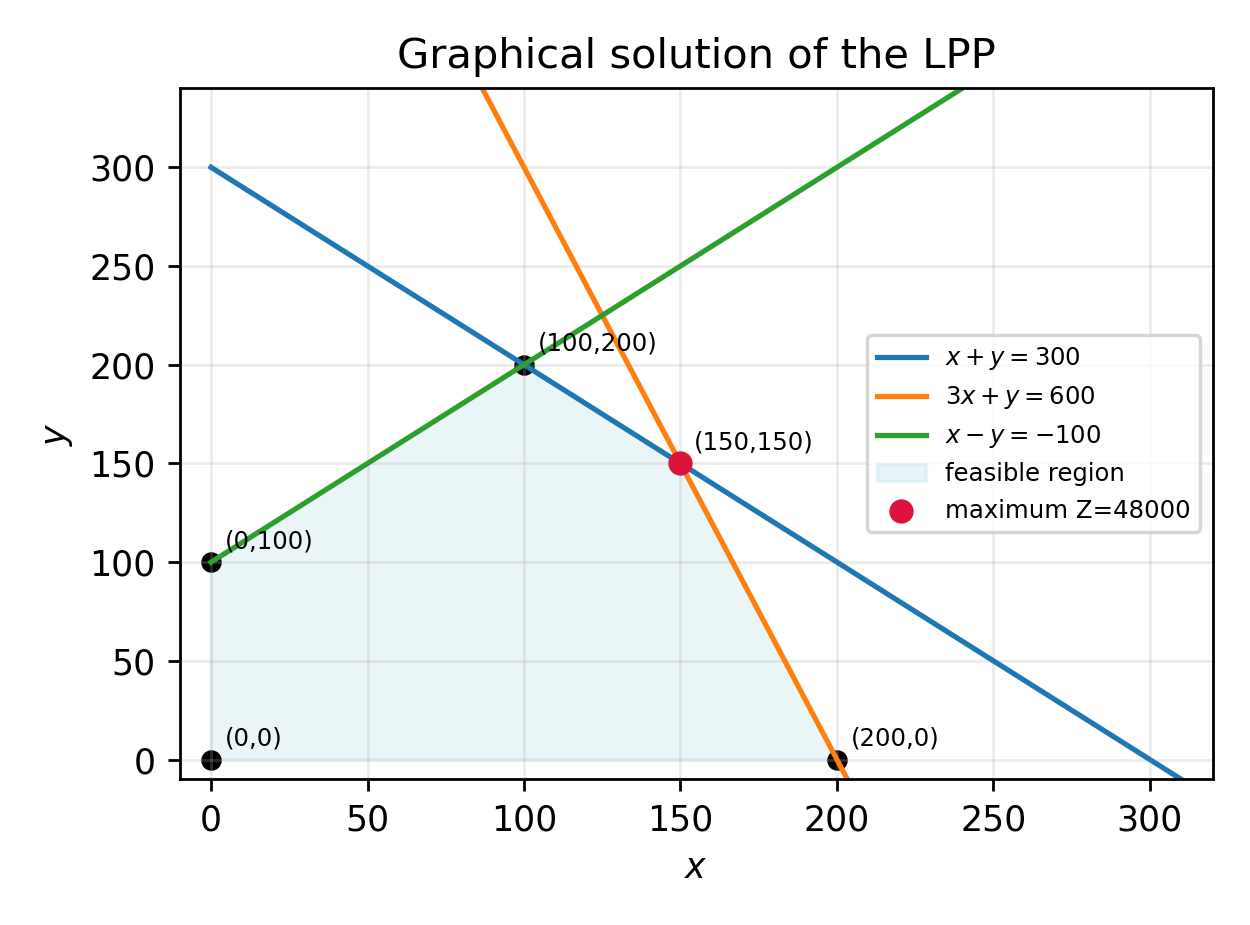
\includegraphics[width=0.68\linewidth]{figs/4.1.29.png}
\caption{Feasible polygon and maximizing vertex for Question 29.}
\end{figure}

\item[4.1.30(a)] Find a point on $\frac{x-2}{3}=\frac{1-y}{2}=\frac{z-3}{2}$ at distance $\sqrt2$ from $(1,2,3)$.

\vspace{0.6em}\par\noindent\textbf{Solution:}

Write a point on the line as $(2+3t,1-2t,3+2t)$. Equating its squared distance from $(1,2,3)$ to $2$ gives $17t^2+10t=0$, so $t=0$ or $t=-10/17$. The points are $\boxed{(2,1,3)}$ and $\boxed{(4/17,37/17,31/17)}$. The code plots the line and both points.
\begin{lstlisting}[frame=single, basicstyle=\rmfamily, escapeinside={(*@}{@*)}]
(*@\makebox[\dimexpr\linewidth-2\fboxsep-2\fboxrule\relax][c]{codes/4.1.30a.py}@*)
\end{lstlisting}
\begin{figure}[H]
\centering
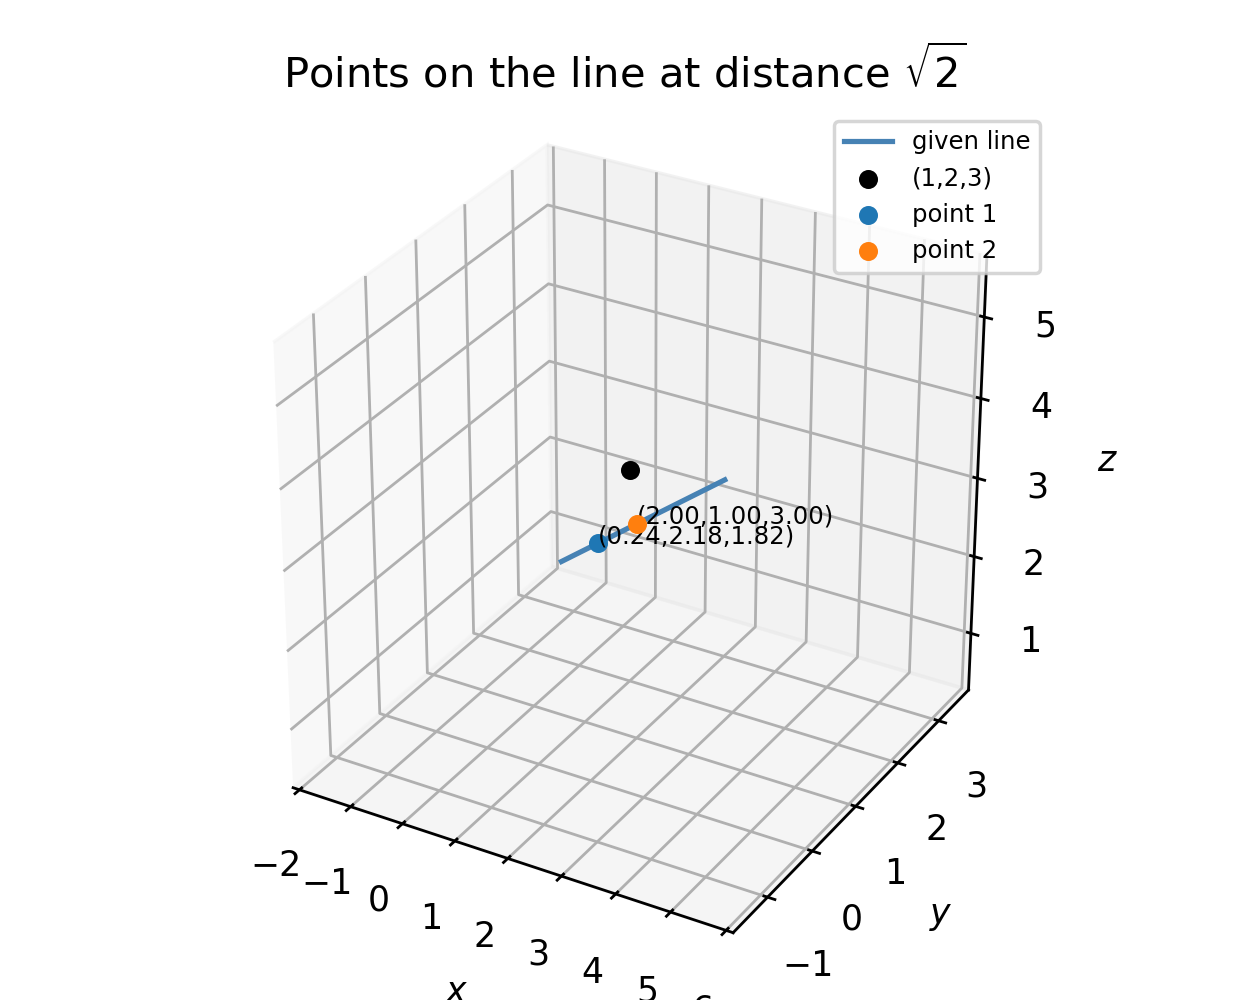
\includegraphics[width=0.65\linewidth]{figs/4.1.30a.png}
\caption{The two points on the line at distance $\sqrt2$.}
\end{figure}

\item[4.1.30(b)] Find the shortest distance between $\vec r=(4+\lambda)\hat i+(2\lambda-1)\hat j-3\lambda\hat k$ and $\vec r=(1+2\mu)\hat i+(4\mu-1)\hat j+(2-5\mu)\hat k$.

\vspace{0.6em}\par\noindent\textbf{Solution:}

Take points $P=(4,-1,0)$ and $Q=(1,-1,2)$ with direction vectors $\vec d_1=(1,2,-3)$ and $\vec d_2=(2,4,-5)$. Then $\vec d_1\times\vec d_2=(2,-1,0)$, and
\[
d=\frac{|(Q-P)\cdot(\vec d_1\times\vec d_2)|}{|\vec d_1\times\vec d_2|}=\frac{6}{\sqrt5}.
\]
The shortest distance is $\boxed{6/\sqrt5}$ units.

\item[4.1.31] A debate is held with probability $1/3$ and a quiz with probability $2/3$. Team A has 4 girls and 6 boys; Team B has 7 girls and 3 boys. Two students are selected from the corresponding team. Find the probability of choosing one girl and one boy.

\vspace{0.6em}\par\noindent\textbf{Solution:}

For Team A the probability is $2(4/10)(6/10)=12/25$. For Team B it is $2(7/10)(3/10)=21/50$. Therefore the required probability is
\[
\frac13\cdot\frac{12}{25}+\frac23\cdot\frac{21}{50}=\boxed{\frac{11}{25}}.
\]

\item[4.1.32(a)] Evaluate $\displaystyle\int\frac{x^2}{(x-1)(x^2+4)}\,dx$.

\vspace{0.6em}\par\noindent\textbf{Solution:}

Partial fractions give $\frac{x^2}{(x-1)(x^2+4)}=\frac{1}{5(x-1)}+\frac{4(x+1)}{5(x^2+4)}$. Hence
\[
\boxed{\int\frac{x^2}{(x-1)(x^2+4)}\,dx=\frac15\ln|x-1|+\frac25\ln(x^2+4)+\frac25\tan^{-1}(x/2)+C}.
\]
The Python code evaluates the decomposition and antiderivative.
\begin{lstlisting}[frame=single, basicstyle=\rmfamily, escapeinside={(*@}{@*)}]
(*@\makebox[\dimexpr\linewidth-2\fboxsep-2\fboxrule\relax][c]{codes/4.1.32a.py}@*)
\end{lstlisting}

\item[4.1.32(b)] Evaluate $\displaystyle\int_0^1\frac{x\tan^{-1}x}{(1+x^2)^{3/2}}\,dx$.

\vspace{0.6em}\par\noindent\textbf{Solution:}

Integration by parts with $u=\tan^{-1}x$ and $dv=x(1+x^2)^{-3/2}dx$ gives
\[
I=-\frac{\pi}{4\sqrt2}+\int_0^1\frac{dx}{(1+x^2)^{3/2}}=\boxed{\frac{4-\pi}{4\sqrt2}}.
\]
The Python code evaluates the exact expression and checks it numerically.
\begin{lstlisting}[frame=single, basicstyle=\rmfamily, escapeinside={(*@}{@*)}]
(*@\makebox[\dimexpr\linewidth-2\fboxsep-2\fboxrule\relax][c]{codes/4.1.32b.py}@*)
\end{lstlisting}

\item[4.1.33] Using integration, find the area enclosed by $y=|x-6|$, the $x$-axis, and $x=4$ to $x=8$.

\vspace{0.6em}\par\noindent\textbf{Solution:}

The graph is V-shaped with vertex $(6,0)$. Thus
\[
\int_4^8|x-6|\,dx=\int_4^6(6-x)\,dx+\int_6^8(x-6)\,dx=2+2=\boxed{4}
\]
square units. The code plots the function and shades the region.
\begin{lstlisting}[frame=single, basicstyle=\rmfamily, escapeinside={(*@}{@*)}]
(*@\makebox[\dimexpr\linewidth-2\fboxsep-2\fboxrule\relax][c]{codes/4.1.33.py}@*)
\end{lstlisting}
\begin{figure}[H]
\centering
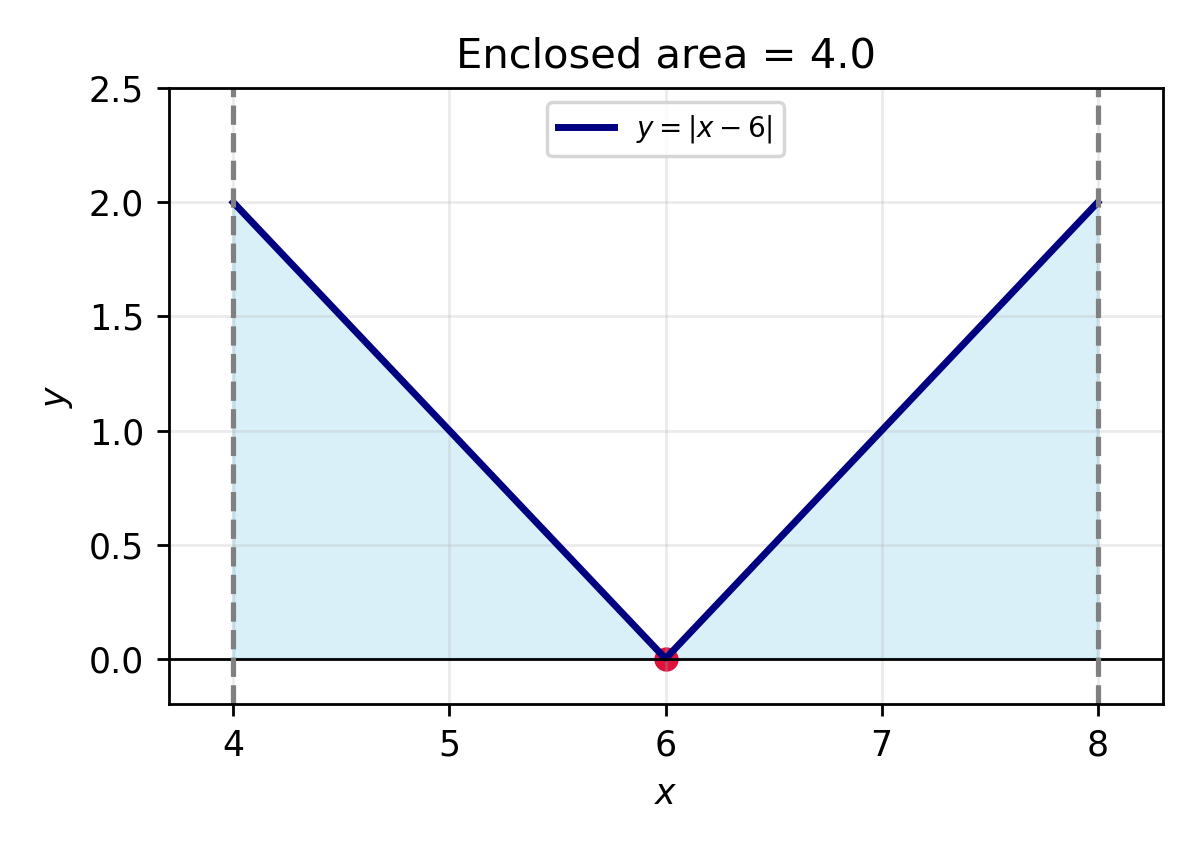
\includegraphics[width=0.65\linewidth]{figs/4.1.33.png}
\caption{Area between $y=|x-6|$ and the $x$-axis on $[4,8]$.}
\end{figure}

\item[4.1.34] Solve $ye^y\,dx=(y^3+2xe^y)\,dy$, given $y(0)=1$.

\vspace{0.6em}\par\noindent\textbf{Solution:}

Treat $x$ as a function of $y$. Dividing by $ye^y$ gives $\frac{dx}{dy}-\frac{2x}{y}=y^2e^{-y}$. The integrating factor is $y^{-2}$, so $\frac{d}{dy}(x/y^2)=e^{-y}$. Integrating and applying $x=0,y=1$ yields $\boxed{x=y^2(e^{-1}-e^{-y})}$.

\item[4.1.35] Find the vector and Cartesian equations of the line through the intersection of $\frac{x-1}{2}=\frac{y-2}{3}=\frac{z-3}{4}$ and $\frac{x-4}{5}=\frac{y-1}{2}=z$, parallel to $3\hat i+2\hat j-8\hat k$.

\vspace{0.6em}\par\noindent\textbf{Solution:}

Parameterizing the two lines and equating coordinates gives their intersection $(-1,-1,-1)$. A line through that point in the required direction is
\[
\boxed{\vec r=(-\hat i-\hat j-\hat k)+t(3\hat i+2\hat j-8\hat k)},\qquad
\boxed{\frac{x+1}{3}=\frac{y+1}{2}=\frac{z+1}{-8}}.
\]
The code plots the two intersecting lines and the required line.
\begin{lstlisting}[frame=single, basicstyle=\rmfamily, escapeinside={(*@}{@*)}]
(*@\makebox[\dimexpr\linewidth-2\fboxsep-2\fboxrule\relax][c]{codes/4.1.35.py}@*)
\end{lstlisting}
\begin{figure}[H]
\centering
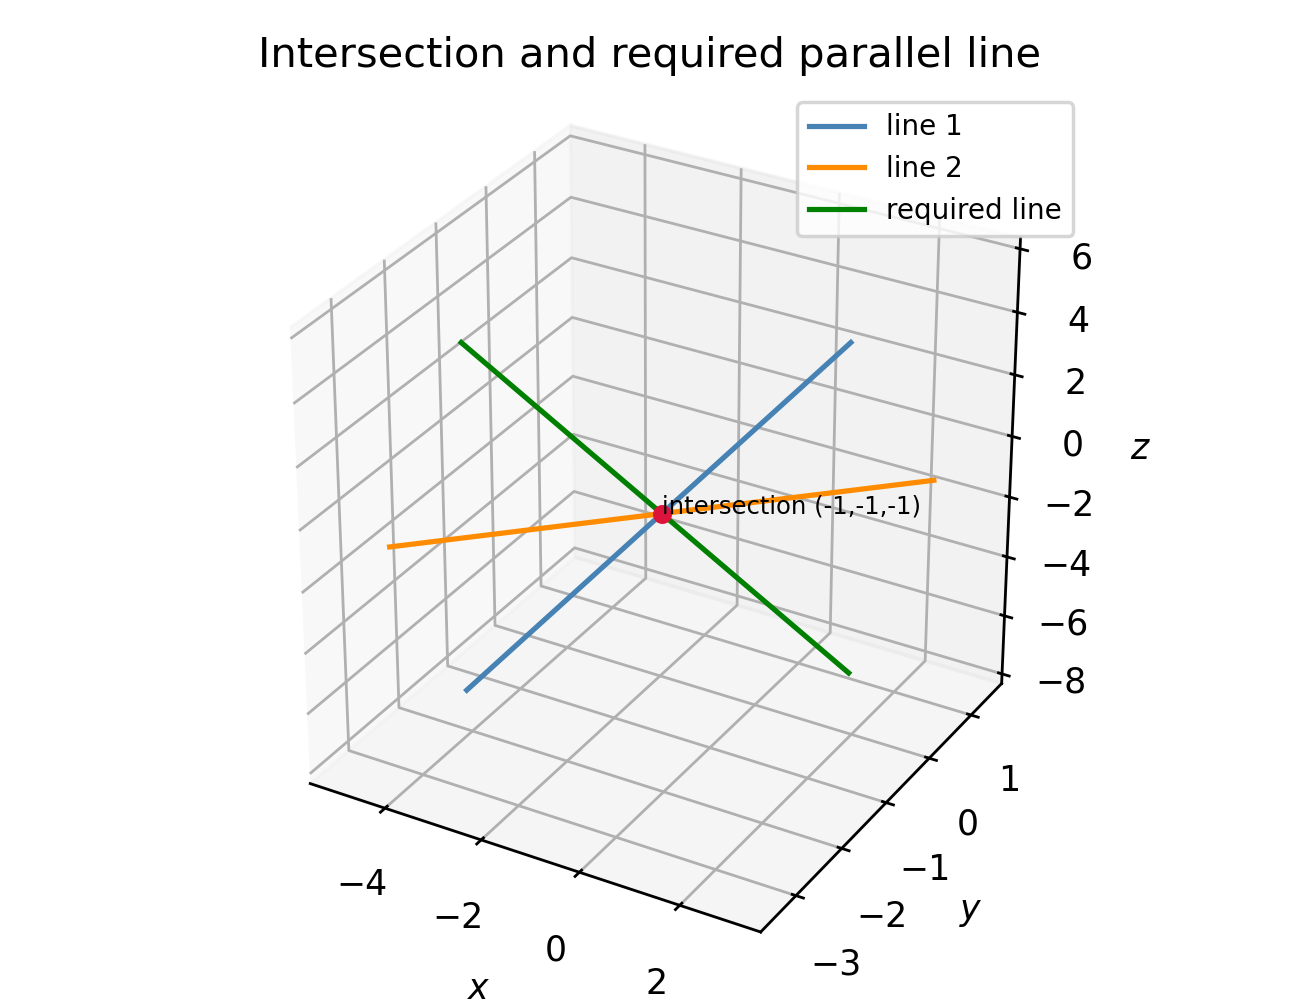
\includegraphics[width=0.65\linewidth]{figs/4.1.35.png}
\caption{The intersecting lines and the parallel line through their intersection.}
\end{figure}

\item[4.1.37] A carpenter designs a cuboid with length $l$, breadth $b$ and height $h$. The conditions are $l+b=h+3$, $2l+3b+h=10$, and $b+7h=3l-1$. (i) Write $AX=B$. (ii) Determine whether $A^{-1}$ exists. (iii)(a) Find $A^{-1}$, or (b) find $A^2+7I$.

\vspace{0.6em}\par\noindent\textbf{Solution:}

The equations give
\[
A=\begin{bmatrix}1&1&-1\\2&3&1\\-3&1&7\end{bmatrix},\quad
X=\begin{bmatrix}l\\b\\h\end{bmatrix},\quad
B=\begin{bmatrix}3\\10\\-1\end{bmatrix}.
\]
$\det A=-8\ne0$, so $A^{-1}$ exists. Solving gives $(l,b,h)=(3,1,1)$ cm. For part (a),
\[
A^{-1}=\begin{bmatrix}-5/2&1&-1/2\\17/8&-1/2&3/8\\-11/8&1/2&-1/8\end{bmatrix};
\]
for part (b),
\[
A^2+7I=\begin{bmatrix}13&3&-7\\5&19&8\\-22&7&60\end{bmatrix}.
\]
The Python code computes the dimensions, determinant, inverse and alternative matrix expression.
\begin{lstlisting}[frame=single, basicstyle=\rmfamily, escapeinside={(*@}{@*)}]
(*@\makebox[\dimexpr\linewidth-2\fboxsep-2\fboxrule\relax][c]{codes/4.1.37.py}@*)
\end{lstlisting}

\item[4.1.38] Three boxes are selected with probabilities $i/6$ for Box $i$, $i=1,2,3$. Box I has 30 red caps, Box II has 20 red and 10 green caps, and Box III has 30 green caps. Find (i) the probability of a red cap; (ii) the probability the cap came from Box II, given that it is green.

\vspace{0.6em}\par\noindent\textbf{Solution:}

(i) $P(R)=\frac16(1)+\frac13(\frac23)+\frac12(0)=\boxed{\frac7{18}}$. (ii) The probability of green is $\frac13(\frac13)+\frac12(1)=\frac{13}{18}$. Hence Bayes' theorem gives $P(\text{II}\mid G)=\frac{(1/3)(1/3)}{13/18}=\boxed{\frac4{13}}$.
\end{list}

\end{document}
